\documentclass[border=5pt]{standalone}
\usepackage[utf8]{inputenc}
\usepackage{amsmath}
\usepackage{tikz}
\usetikzlibrary{positioning, fit, shapes}
\usetikzlibrary{chains}
\usetikzlibrary{calc}
\usetikzlibrary{decorations.pathmorphing}
\usetikzlibrary{shapes.multipart}
\usetikzlibrary{decorations,arrows}
\usetikzlibrary{decorations.pathmorphing}
\usepgflibrary{decorations.pathreplacing} 

\begin{document}

\begin{tikzpicture}[node distance=0cm, font=\sffamily]

% Master
\node at (0, 0) {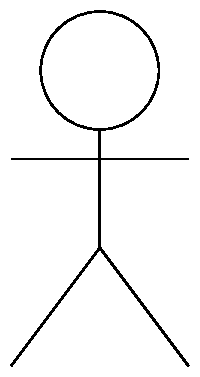
\includegraphics{Stickman.pdf}};
\node at (0, 2) {Master};

% Minions
\node[opacity=0] at (5, 0) {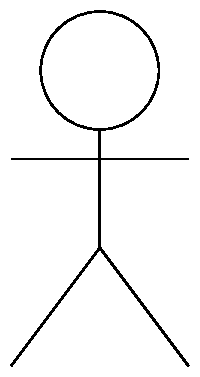
\includegraphics[scale=0.4]{Stickman.pdf}};
\node[opacity=0] at (5, 1.6) {Working};
\node[opacity=0] at (5, 3.5) {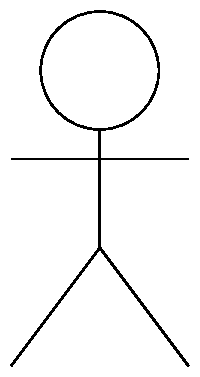
\includegraphics[scale=0.4]{Stickman.pdf}};
\node[opacity=0] at (5, 5.1) {Working};
\node[opacity=0] at (5, -3.5) {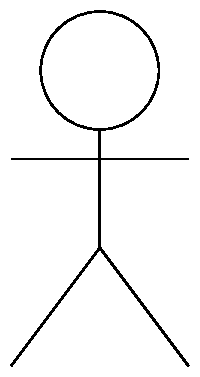
\includegraphics[scale=0.4]{Stickman.pdf}};
\node[opacity=0] at (5, -1.9) {Working};

% Spawn arrows
\node[opacity=0] at (3, 0.4) {Spawn};
\node[scale=2, opacity=0] at (3, 3) {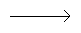
\includegraphics{RArrow.pdf}};
\node[opacity=0] at (3, 3.4) {Spawn};
\node[scale=2, opacity=0] at (3, 0) {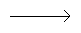
\includegraphics{RArrow.pdf}};
\node[opacity=0] at (3, -2.6) {Spawn};
\node[scale=2, opacity=0] at (3, -3) {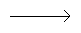
\includegraphics{RArrow.pdf}};

\end{tikzpicture}

\end{document}
